% \iffalse meta-comment
%
% File: litetable.dtx
% -----------------------------------------------------------------------
%   Copyright (C) 2023-2025 by Mingyu Xia <myhsia@outlook.com>          *
%                                                                       *
%   This work may be distributed and/or modified under the conditions   *
%   of the LaTeX Project Public License (LPPL), either version 1.3c of  *
%   this license or (at your option) any later version.                 *
%   The latest version of this license is in                            *
%                                                                       *
%       http://www.latex-project.org/lppl.txt                           *
%                                                                       *
%   and version 1.3c or later is part of all distributions of LaTeX     *
%   version 2008 or later.                                              *
%                                                                       *
%   This work has the LPPL maintenance status `maintained'.             *
%                                                                       *
%   The Current Maintainer of this work is Mingyu Xia.                  *
%                                                                       *
%   This work consists of the files litetable.dtx,                      *
%                                   litetable.ins,                      *
%                 the derived files litetable.sty,                      *
%           the documentation files litetable.pdf,                      *
%                               and README.md.                          *
% -----------------------------------------------------------------------
%
%   Any modification of this file should ensure that the copyright and
%   license information is placed in the derived files.
%
% -----------------------------------------------------------------------
%
%<*internal>
\iffalse
%</internal>
%
%<*readme>
[![CTAN Version](https://img.shields.io/ctan/v/litetable)](https://ctan.org/pkg/litetable)
[![GitHub Release](https://img.shields.io/github/v/release/myhsia/litetable)](https://github.com/myhsia/litetable/releases/latest)
[![GitHub Last Commit](https://img.shields.io/github/last-commit/myhsia/litetable)](https://github.com/myhsia/litetable/commits)
[![Actions Status](https://github.com/myhsia/litetable/actions/workflows/main.yaml/badge.svg?branch=main)](https://github.com/myhsia/litetable/actions)
[![GitHub Repo stars](https://img.shields.io/github/stars/myhsia/litetable)](https://github.com/myhsia/litetable)

The `litetable` Package
=======================

The `litetable` package (conducted with LaTeX3) provides a colorful design
of timetable.

Overview
--------

The package provides the `\course` macro

    \course [<keys>] {<start num>} [<keys>] {<end-num>} [<keys>]

to add colorful custom course block.

See `litetable.pdf` for more. Happy TeXing!

Issues
------

The issue tracker for `litetable` is currently located
[on GitHub](https://github.com/myhsia/litetable/issues).

Build status
------------

This project uses [GitHub Actions](https://github.com/features/actions)
as a hosted continuous integration service. For each commit, the build status
is tested using the current release of TeX Live.

_Current build status:_ ![build status](https://github.com/myhsia/litetable/actions/workflows/main.yaml/badge.svg?branch=main)

Copyright and License
---------------------

Copyright (C) 2023-2025 by Mingyu Xia <myhsia@outlook.com>

This work may be distributed and/or modified under the conditions
of the LaTeX Project Public License (LPPL), either version 1.3c of
this license or (at your option) any later version.
The latest version of this license is in

    http://www.latex-project.org/lppl.txt

and version 1.3c or later is part of all distributions of LaTeX
version 2008 or later.

This work has the LPPL maintenance status `maintained'.

The Current Maintainer of this work is **Mingyu Xia**.
%</readme>
%
%<*internal>
\fi
%</internal>
%
%<*driver>
\documentclass[svgnames]{l3doc}
\usepackage{pdfpages, twemojis}
\usepackage[mono = false]{libertine}
\AddToHook{env/function/before}{\vspace*{-.7\baselineskip}}
\AddToHook{env/syntax/after}   {\par\vspace*{.2\baselineskip}}
\makeatletter
\def \@key  #1{\textcolor{red}{\textbf{\texttt{#1}}}\:\texttt{=}\:}
\def \s@key #1{\textcolor{red}{\texttt{\textup{\textbf{#1}}}}}
\DeclareDocumentCommand \key s {\IfBooleanTF{#1}\s@key\@key}
\DeclareCommandCopy \val \meta
\def \TFF {true\textup{\textbar \textbf{false}}}
\def \TTF {\textup{\textbf{true}\textbar} false}
\def \HoLogo@ApLaTeX #1{^^A
  \HOLOGO@mbox {A\kern -.05em p\kern -.05em \hologo{LaTeX}}}
\makeatother
\newlist{keyval}{itemize}{10}
\setlist[keyval]{leftmargin = 0pt, labelsep = 0pt}
\makeindex
\begin{document}
  \DocInput{\jobname.dtx}
\end{document}
%</driver>
% \fi
%
% \title{^^A
%   The \cls{litetable} Package --- Colorful Timetable\thanks{^^A
%     \url{https://github.com/myhsia/litetable},
%     \url{https://ctan.org/pkg/litetable}^^A
%   }^^A
% }
%
% \author{^^A
%   Mingyu Xia \texttt{<^^A
%     \href{mailto:myhsia@outlook.com}{myhsia@outlook.com}^^A
%     \texorpdfstring{\:\textbar\:}{, }^^A\href{mailto:xiamingyu@westlake.edu.cn}
%     {xiamingyu@westlake.edu.cn}>^^A
%   }\thanks{^^A
%     \href{https://github.com/ljguo1020}{Lijun Guo} developed an interface
%     to parse \meta{left} \texttt{->} \meta{right} data structures.^^A
%   }^^A
% }
%
% \date{Released 2025-07-20\quad \texttt{v3.5A}}
%
% \maketitle
%
% \begin{documentation}
%
% \section{Introduction}
%
% The \cls{litetable} package provides a colorful design of timetable, developed
% by \pkg{expl3} based on \pkg{tikz}. It supports various compilation methods,
% such as \hologo{pdfLaTeX}, \hologo{XeLaTeX}, \hologo{ApLaTeX},
% \hologo{LuaLaTeX}, etc. Click to jump to the manual's
% \href{http://mirrors.ctan.org/macros/latex/contrib/litetable/litetable-zh-cn.pdf}{[\textsf{Chinese Version}]}
% \href{http://mirrors.ctan.org/macros/latex/contrib/litetable/litetable-zh-hk.pdf}{[\textsf{Cantonese Version}]}.
%
% \section{Usage}
%
% To load this package, write the line
% \begin{quote}
%   |\usepackage{litetable}|
% \end{quote}
%
% \DescribeEnv{litetable}
% The \env{litetable} environment can create a blank timetable frame, and it
% should be executed after commands \cs{timelist} and \cs{weeklist}.
% \begin{quote}
%   |\begin{litetable}|
%     \oarg{keys} \marg{title} \oarg{keys}| ... |
%   |\end{litetable}|
% \end{quote}
% The mandatory argument can set the title of the timetable, and the
% optional argument accepts the following keys
% \begin{keyval}
%   \item [\key{color}] \val{string} can set the background color
%   (Default: |gray|), this key's name could be omitted.
%   \item [\key{sem}] \val{string} can set the semester information at the
%   northeast corner of the page.
%   \item [\key{hline}] \val{string} can set style of the horizontal lines
%   (Default: |solid|).
% \end{keyval}
%
% \begin{function}{\weeklist}
%   \begin{syntax}
%     \cs{weeklist} \oarg{keys} \marg{list} \oarg{keys}
%   \end{syntax}
%   The mandatory argument accepts an array to set a list of working days and
%   the width of each column at the top of the timetable.
%   The optional argument accepts the following keys
%   \begin{keyval}
%     \item [\key{format}] \val{format commands} can set the font for the list
%     of working days (Default: |\bfseries|).
%     \item [\key{sep}] \val{dim} can set the separator of
%     the list of working days.
%   \end{keyval}
%   \begin{verbatim}
%     \weeklist [ format = \bfseries \scshape, sep = \textbar ]
%       { Mon -> 1.05, Tue -> 1.05, Wed -> 1.1, Thu -> 1.1, Fri -> .9 }
%   \end{verbatim}
% \end{function}
%
% \begin{function}{\timelist}
%   \begin{syntax}
%     \cs{timelist} \oarg{keys} \marg{list} \oarg{keys}
%   \end{syntax}
%   The mandatory argument accepts an array to set the time list on the left
%   side of the timetable. The optional argument accepts the following keys
%   \begin{keyval}
%     \item [\key{numformat}] \val{format commands} can set the font for the
%     sequence number of the time list
%     (Default: |\ttfamily \bfseries|).
%     \item [\key{timefont}] \val{format commands} can set the font for the time
%     of the time list. (Default: |\ttfamily|).
%     \item [\key{hidetime}] \val{\TFF} hide the time in the time list and only
%     retain the sequence number. The initial value is |false|.
%   \end{keyval}
%   \begin{verbatim}
%     \timelist [ numformat = \bfseries, timeformat = \ttfamily ]
%       { 08:30 -> 10:00, 10:30 -> 12:00, 13:00 -> 14:30, 15:00 -> 16:30 }
%   \end{verbatim}
% \end{function}
%
% \begin{function}{\course}
%   \begin{syntax}
%     \cs{course} \oarg{keys} \marg{start} \oarg{keys} \marg{end} \oarg{keys}
%   \end{syntax}
%   It's used to add course boxes on the current workday, and needs to be
%   executed within the \env{litetable} environment.
%   The two mandatory arguments can set the start and ends of the course
%   respectively, the optional argument accepts the following keys
%   \begin{keyval}
%     \item [\key{color}] \val{string} can set the color of the course box
%     (Default: |teal|), this key's name could be omitted.
%     \item [\key{subject}] \val{string} can set the name of the course.
%     \item [\key{location}] \val{string} can set the location of the course.
%     \item [\key{lecture}] \val{string} can set the lecture of the course.
%     \item [\key{comment}] \val{string} can add footnote to the course.
%   \end{keyval}
%   \begin{texnote}
%     \begin{itemize}[leftmargin = 2em]
%       \item If \meta{start} |=| \meta{end} (the height of the
%       course box is $1$ unit), then \key*{location} and \key*{lecture} will be
%       outputted in the same line and \key*{comment} will be hidden.
%       \item The template will correct automatically if \meta{start} and
%       \meta{end} were misplaced.
%       \item If neither \key*{location} nor \key*{lecture} is assigned value,
%       then \key*{subject} will be outputted in the vertical center of the
%       course box.
%       \item Course boxes that exceed the range of the timetable won't
%       display and it will return a warning.
%       The input example refers to Appendix \ref{mwe}.
%     \end{itemize}
%   \end{texnote}
% \end{function}
%
% \begin{function}{\newday}
%   \begin{syntax}
%     \cs{newday} \oarg{integral value}
%   \end{syntax}
%   It can move the next course boxes right \meta{integral value} working days.
%   The default value of the optional argument is |1|.
% \end{function}
%
% \begin{function}{\more}
%   \begin{syntax}
%     \cs{more} \marg{comment}
%   \end{syntax}
%   It can add a comment at the southwest corner of the timetable.
% \end{function}
%
% \appendix \linespread{1.3}
%
% \section{Working Example} \label{mwe}
%
% \verbatiminput{litetable-demo.tex}
%
% 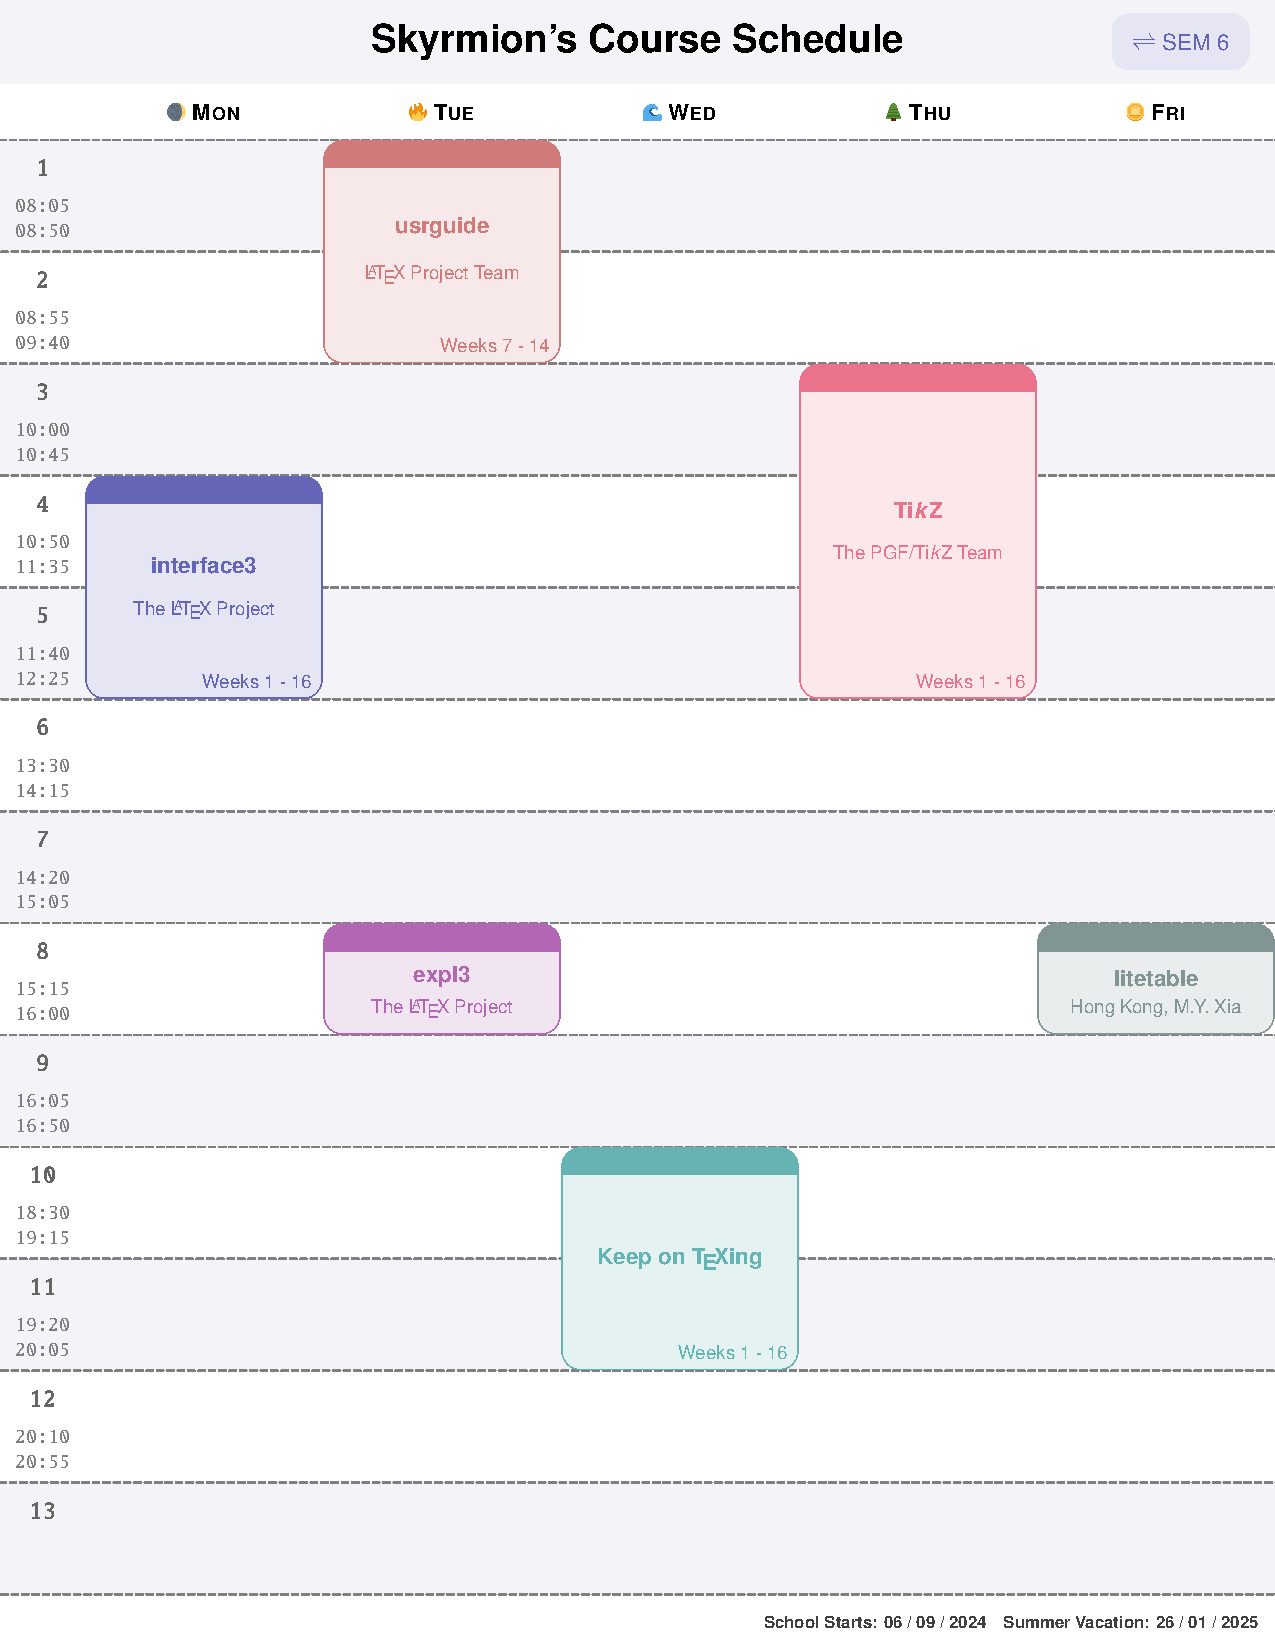
\includepdf{litetable-demo.pdf}
%
% \end{documentation}
%
% \begin{implementation}
% \linespread{1.3}
% \section{The Source Code}
%
%    \begin{macrocode}
%<*package>
%    \end{macrocode}
%
%    \begin{macrocode}
%<@@=ltbl>
%    \end{macrocode}
%
%    \begin{macrocode}
\ProvidesExplPackage {litetable} {2025-07-20} {v3.5A}
  {A Colorful Timetable Design}
%    \end{macrocode}
%
%    \begin{macrocode}
\RequirePackage{tikz}
%    \end{macrocode}
%   Warning Broadcast
%    \begin{macrocode}
\cs_new_protected:Npn \@@_msg_new:nn #1#2
  { \msg_new:nnn { litetable } {#1} {#2} }
\cs_new_protected:Npn \@@_msg_warning:n #1
  { \msg_warning:nn { litetable } {#1} }
\@@_msg_new:nn { course }
  { \exp_not:N \course ~ box(s) ~ exceed ~ workdays ~ were ~ ignored }
%    \end{macrocode}
% \begin{macro}
%   {
%     \@@_get_left:nN, \@@_get_right:nN,
%     \@@_get_left:eN, \@@_get_right:eN,
%   }
%   Handle \meta{left} |->| \meta{right} data structures
%   (by \href{https://github.com/ljguo1020}{Lijun Guo})
%    \begin{macrocode}
\cs_new_protected_nopar:Npn \@@_get_left:nN #1#2
  {
    \group_begin: \seq_set_split:Nnn \l_@@_tmpa_seq { -> } {#1}
    \exp_args:NNNe \group_end:
    \tl_set:Nn #2 { \seq_item:Nn \l_@@_tmpa_seq { 1 } }
  }
\cs_new_protected_nopar:Npn \@@_get_right:nN #1#2
  {
    \group_begin: \seq_set_split:Nnn \l_@@_tmpa_seq { -> } {#1}
    \exp_args:NNNe \group_end:
    \tl_set:Nn #2 { \seq_item:Nn \l_@@_tmpa_seq { 2 } }
  }
\cs_generate_variant:Nn \@@_get_left:nN  { eN }
\cs_generate_variant:Nn \@@_get_right:nN { eN }
%    \end{macrocode}
% \end{macro}
%
% \subsection{User's Interface}
%
% \begin{macro}{\weeklist}
%   Set a list of working days and the width of each column at the top of the
%   timetable.
%    \begin{macrocode}
\NewDocumentCommand \weeklist { O{} m O{} }
  {
    \keys_set:nn { litetable / weeklist } { #1, #3 }
    \@@_weeklist:n {#2}
  }
%    \end{macrocode}
% \begin{variable}{\l_@@_weeklist_format_tl, \l_@@_weeklist_sep_tl}
%   Key--value definitions for the \cs{weeklist} command.
%    \begin{macrocode}
\keys_define:nn { litetable / weeklist }
  {
    format   .tl_set:N  = \l_@@_weeklist_format_tl,
      format .initial:n = \bfseries,
    sep      .tl_set:N  = \l_@@_weeklist_sep_tl
  }
%    \end{macrocode}
% \end{variable}
% \end{macro}
% \begin{macro}{\timelist}
%   Set the time list on the left side of the timetable.
%    \begin{macrocode}
\NewDocumentCommand \timelist { O{} m O{} }
  {
    \keys_set:nn { litetable / timelist } { #1, #3 }
    \@@_timelist:n {#2}
  }
%    \end{macrocode}
% \begin{variable}
%   {
%     \l_@@_timelist_numformat_tl,  \l_@@_timelist_timeformat_tl,
%     \l_@@_timelist_hidetime_bool
%   }
%   Key--value definitions for the \cs{timelist} command.
%    \begin{macrocode}
\keys_define:nn { litetable / timelist }
  {
    numformat    .tl_set:N   = \l_@@_timelist_numformat_tl,
      numformat  .initial:n  = \ttfamily \bfseries,
    timeformat   .tl_set:N   = \l_@@_timelist_timeformat_tl,
      timeformat .initial:n  = \ttfamily,
    hidetime     .bool_set:N = \l_@@_timelist_hidetime_bool,
      hidetime   .initial:n  = false,
      hidetime   .default:n  = true
  }
%    \end{macrocode}
% \end{variable}
% \end{macro}
% \begin{environment}{litetable}
%   Create a blank timetable frame.
%    \begin{macrocode}
\NewDocumentEnvironment { litetable } { O{} m O{} }
  {
    \clearpage \thispagestyle{empty}
    \tikzpicture [ remember~picture, overlay ]
    \group_begin:
    \keys_set:nn { litetable / frame } { #1, #3 }
    \@@_maketable:n {#2}
  } { \group_end: \endtikzpicture \clearpage }
%    \end{macrocode}
% \begin{variable}{\l_@@_bg_color_tl, \l_@@_bg_sem_tl}
%   Key--value definitions for the \env{litetable} command.
%    \begin{macrocode}
\keys_define:nn { litetable / frame }
  {
    color   .tl_set:N  = \l_@@_bg_color_tl,
      color .initial:n = gray,
    hline   .tl_set:N  = \l_@@_hline_type_tl,
      hline .initial:n = solid,
    sem     .tl_set:N  = \l_@@_bg_sem_tl,
    unknown .code:n    = \tl_if_novalue:nF {#1}
      { \tl_set_eq:NN \l_@@_bg_color_tl \l_keys_key_tl }
  }
%    \end{macrocode}
% \end{variable}
% \end{environment}
% \begin{macro}{\course}
%   Add course boxes on the current workday
%    \begin{macrocode}
\NewDocumentCommand \course { O{} m O{} m O{} }
  {
    \group_begin:
    \bool_lazy_any:nTF
      {
        {
          \int_compare_p:nNn { \l_@@_weekday_int } >
            { \clist_count:N \l_@@_week_clist }
        }
        { \int_compare_p:nNn {#2} > { \clist_count:N \l_@@_time_clist } }
        { \int_compare_p:nNn {#4} > { \clist_count:N \l_@@_time_clist } }
      } { \@@_msg_warning:n { course } }
      {
        \keys_set:nn { litetable / course } { #1, #3, #5 }
        \int_compare:nNnTF {#2} < {#4}
          { \@@_course_box_aux:nn {#2} {#4} }
          { \@@_course_box_aux:nn {#4} {#2} }
      }
    \group_end:
  }
%    \end{macrocode}
% \begin{variable}
%   {
%     \l_@@_course_color_tl   , \l_@@_course_subject_tl,
%     \l_@@_course_lecture_tl , \l_@@_course_lecture_tl,
%     \l_@@_course_location_tl, \l_@@_course_comment_tl
%   }
%   Key--value definitions for the \cs{course} command.
%    \begin{macrocode}
\keys_define:nn { litetable / course }
  {
    color    .tl_set:N  = \l_@@_course_color_tl,
      color  .initial:n = black,
    subject  .tl_set:N  = \l_@@_course_subject_tl,
    lecture  .tl_set:N  = \l_@@_course_lecture_tl,
    location .tl_set:N  = \l_@@_course_location_tl,
    comment  .tl_set:N  = \l_@@_course_comment_tl,
    unknown  .code:n    = \tl_if_novalue:nF {#1}
      { \tl_set_eq:NN \l_@@_course_color_tl \l_keys_key_tl }
  }
%    \end{macrocode}
% \end{variable}
% \end{macro}
% \begin{macro}{\more}
%   Add a comment at the southwest corner of the timetable.
%    \begin{macrocode}
\NewDocumentCommand \more { m }
  {
    \node [ yshift = .5\l_@@_time_vunit_dim, left = 1ex,
            darkgray, font = \small \bfseries
          ] at (current~page.south~east) {#1};
  }
%    \end{macrocode}
% \end{macro}
% \begin{macro}{\newday}
%   Move the next course boxes right \meta{integral value} working days.
%    \begin{macrocode}
\NewDocumentCommand \newday { O{1} } { \int_add:Nn \l_@@_weekday_int {#1} }
\int_new:N \l_@@_weekday_int
\int_set:Nn \l_@@_weekday_int { 1 }
%    \end{macrocode}
% \end{macro}
%
% \subsection{Internal Auxiliary}
%
% \begin{variable}
%   {
%     \l_@@_week_ratio_clist, \l_@@_week_accum_clist,
%     \l_@@_week_num_fp     , \l_@@_week_hunit_dim
%   }
%   The ratios of every working days, the accumulation of the ratios of every
%   working days, the sequence number of every working days, the horizontal
%   width unit of the timetable.
%    \begin{macrocode}
\clist_new:N \l_@@_week_ratio_clist
\clist_new:N \l_@@_week_accum_clist
\fp_new:N \l_@@_week_num_fp
\dim_new:N \l_@@_week_hunit_dim
%    \end{macrocode}
% \end{variable}
% \begin{macro}{\@@_weeklist:n}
%   Define the auxiliary command of \cs{weeklist}.
%    \begin{macrocode}
\cs_new_protected_nopar:Npn \@@_weeklist:n #1
  {
    \clist_set:Nn \l_@@_week_clist {#1}
    \exp_args:NNf \clist_map_inline:Nn \l_@@_week_clist
      {
        \@@_get_right:eN {##1} \l_@@_tmpb_tl
        \clist_put_right:Ne \l_@@_week_ratio_clist { \l_@@_tmpb_tl }
      }
    \int_step_inline:nn { \clist_count:N \l_@@_week_clist }
      {
        \clist_clear:N \l_@@_week_accumtmp_clist
        \int_step_inline:nn {##1}
          {
            \clist_put_right:Ne \l_@@_week_accumtmp_clist
              { \clist_item:Nn \l_@@_week_ratio_clist {####1} }
          }
        \clist_put_right:Ne \l_@@_week_accum_clist
          { \fp_eval:n { \clist_use:Nn \l_@@_week_accumtmp_clist { + } } }
      }
    \fp_set:Nn \l_@@_week_num_fp
      {
        \clist_item:Nn \l_@@_week_accum_clist
          { \clist_count:N \l_@@_week_clist }
      }
    \dim_set:Nn \l_@@_week_hunit_dim
      { \fp_eval:n { 14/\l_@@_week_num_fp/15 } \paperwidth }
  }
%    \end{macrocode}
% \end{macro}
% \begin{variable}{\l_@@_time_num_int, \l_@@_time_vunit_dim}
%   The sequence number of the time list, and the vertical gap between the
%   start and end time.
%    \begin{macrocode}
\int_new:N \l_@@_time_num_int
\dim_new:N \l_@@_time_vunit_dim
%    \end{macrocode}
% \end{variable}
% \begin{macro}{\@@_timelist:n}
%   Define the auxiliary command of \cs{timelist}.
%    \begin{macrocode}
\cs_new_protected_nopar:Npn \@@_timelist:n #1
  {
    \clist_set:Nn \l_@@_time_clist {#1}
    \int_set:Nn \l_@@_time_num_int { \clist_count:N \l_@@_time_clist }
    \dim_set:Nn \l_@@_time_vunit_dim
      { \fp_eval:n { 1/(2\l_@@_time_num_int + 3.5) } \paperheight }
  }
%    \end{macrocode}
% \end{macro}
% \begin{variable}{\l_@@_timelist_shift_dim}
%   Store the vertical shift of the sequence number of the time list.
%    \begin{macrocode}
\dim_new:N \l_@@_timelist_shift_dim
%    \end{macrocode}
% \end{variable}
% \begin{macro}{\@@_maketable:n}
%   Define the auxiliary command of the \env{litetable} environment.
%    \begin{macrocode}
\cs_new_protected_nopar:Npn \@@_maketable:n #1
  {
    \fill [ \l_@@_bg_color_tl!5 ]
      (current~page.north~west) rectangle +
      (\paperwidth, -1.5\l_@@_time_vunit_dim)
     node [ midway, black, font = \huge \bfseries ] {#1};
    \tl_if_empty:NF \l_@@_bg_sem_tl
      {
        \node [ shift = {(-.02\paperwidth, -.75\l_@@_time_vunit_dim)},
                left, rectangle, fill = DarkBlue!10, text = DarkBlue!60,
                inner~sep = 2ex, rounded~corners = 8pt, font = \large
              ] at (current~page.north~east) { \l_@@_bg_sem_tl };
      }
    \int_step_inline:nnnn { 0 } { 2 } { \l_@@_time_num_int }
      {
        \filldraw [ fill = \l_@@_bg_color_tl!5, thick,
                    draw = gray, \l_@@_hline_type_tl ]
          ([shift =
            {(-.4pt, \fp_eval:n { -2 * ##1 - 2.5 } \l_@@_time_vunit_dim)}
           ]current~page.north~west
          ) rectangle + (\paperwidth + .8pt, -2\l_@@_time_vunit_dim);
      }
    \bool_if:NTF \l_@@_timelist_hidetime_bool
      {
        \dim_set:Nn \l_@@_timelist_shift_dim
          { -1.5\l_@@_time_vunit_dim }
      }
      {
        \dim_set:Nn \l_@@_timelist_shift_dim
          { -\l_@@_time_vunit_dim }
      }
    \int_step_inline:nn { \l_@@_time_num_int }
      {
        \node [ darkgray!80, shift =
                {(
                  \paperwidth/30,
                  -2 * ##1 \l_@@_time_vunit_dim +
                  \l_@@_timelist_shift_dim
                )}, font = \large \l_@@_timelist_numformat_tl
              ] at (current~page.north~west) {##1};
      }
    \bool_if:NF \l_@@_timelist_hidetime_bool
      {
        \int_step_inline:nn { \clist_count:N \l_@@_time_clist }
          {
            \@@_get_left:eN  { \clist_item:Nn \l_@@_time_clist {##1} }
              \l_@@_tmpa_tl
            \@@_get_right:eN { \clist_item:Nn \l_@@_time_clist {##1} }
              \l_@@_tmpb_tl
            \node [ gray, align = center, shift =
                    {(
                      \paperwidth/30,
                      \fp_eval:n { -1.85 - 2 * ##1 } \l_@@_time_vunit_dim
                    )}, font = \l_@@_timelist_timeformat_tl
                  ] at (current~page.north~west)
              { \l_@@_tmpa_tl\\ \l_@@_tmpb_tl };
          }
      }
    \int_step_inline:nn { \clist_count:N \l_@@_week_clist }
      {
        \int_compare:nNnF {##1} = { \clist_count:N \l_@@_week_clist }
          {
            \node [ shift =
                    {(\fp_eval:n
                        {
                          14 * \clist_item:Nn \l_@@_week_accum_clist {##1}/
                          \l_@@_week_num_fp/15 + 1/15
                        } \paperwidth, -2\l_@@_time_vunit_dim
                    )}, darkgray, font = \ttfamily
                  ] at (current~page.north~west) { \l_@@_weeklist_sep_tl };
          }
        \@@_get_left:eN { \clist_item:Nn \l_@@_week_clist {##1} }
          \l_@@_tmpa_tl
        \node [ shift =
                {(\fp_eval:n
                    {
                      14(
                        \clist_item:Nn \l_@@_week_accum_clist {##1} -
                        \clist_item:Nn \l_@@_week_ratio_clist {##1}/2
                        )/\l_@@_week_num_fp/15 + 1/15
                    } \paperwidth, -2\l_@@_time_vunit_dim
                )}, font = \large \l_@@_weeklist_format_tl
              ] at (current~page.north~west) { \l_@@_tmpa_tl };
      }
  }
%    \end{macrocode}
% \end{macro}
% \begin{variable}{\l_@@_course_shift_dim}
%   Store the vertical shift of the course subject in course box.
%    \begin{macrocode}
\dim_new:N \l_@@_course_shift_dim
%    \end{macrocode}
% \end{variable}
% \begin{macro}{\@@_course_box_aux:nn}
%   Define the auxiliary command of \cs{course}.
%    \begin{macrocode}
\cs_new_protected_nopar:Npn \@@_course_box_aux:nn #1#2
  {
    \begin{scope}
      \clip [ preaction = { draw, ultra~thick, \l_@@_course_color_tl!60 },
              preaction = { fill, \l_@@_course_color_tl!10 },
              rounded~corners = 8pt ]
        ([shift =
          {(
            \fp_eval:n
              {
                \clist_item:Nn \l_@@_week_accum_clist
                  { \l_@@_weekday_int } -
                \clist_item:Nn \l_@@_week_ratio_clist
                  { \l_@@_weekday_int }
              } \l_@@_week_hunit_dim + \paperwidth/15 + 1.2pt,
            \fp_eval:n { -.5 - 2 * #1 } \l_@@_time_vunit_dim - 1.2pt
        )}]current~page.north~west) rectangle +
        (
          \clist_item:Nn \l_@@_week_ratio_clist
            { \l_@@_weekday_int } \l_@@_week_hunit_dim - 2.4pt,
          \fp_eval:n { 2(#1 - #2 - 1) } \l_@@_time_vunit_dim + 2.4pt
        );
      \fill [ \l_@@_course_color_tl!60 ]
        ([shift =
          {(
            \fp_eval:n
              {
                \clist_item:Nn \l_@@_week_accum_clist
                  { \l_@@_weekday_int } -
                \clist_item:Nn \l_@@_week_ratio_clist
                  { \l_@@_weekday_int }
              } \l_@@_week_hunit_dim + \paperwidth/15,
            \fp_eval:n { -.5 - 2 * #1 } \l_@@_time_vunit_dim
        )}]current~page.north~west) rectangle +
        (
          \clist_item:Nn \l_@@_week_ratio_clist
            { \l_@@_weekday_int } \l_@@_week_hunit_dim,
          -\l_@@_time_vunit_dim/2
        );
    \end{scope}
    \int_compare:nNnTF {#1} = {#2}
      {
        \bool_lazy_and:nnTF
          { \tl_if_empty_p:N \l_@@_course_location_tl   }
          { \tl_if_empty_p:N \l_@@_course_lecture_tl    }
          { \tl_set:Nn \l_@@_course_anchor_tl {       } }
          { \tl_set:Nn \l_@@_course_anchor_tl { above } }
        \node
          [ \l_@@_course_anchor_tl, \l_@@_course_color_tl!60, shift =
            {(
              \fp_eval:n
                {
                  \clist_item:Nn \l_@@_week_accum_clist
                    { \l_@@_weekday_int } -
                  \clist_item:Nn \l_@@_week_ratio_clist
                    { \l_@@_weekday_int }/2
                } \l_@@_week_hunit_dim + \paperwidth/15,
              \fp_eval:n { -1.75 - #1 - #2 } \l_@@_time_vunit_dim
            )}, align = center, font = \bfseries
          ] at (current~page.north~west) { \l_@@_course_subject_tl };
        \bool_lazy_or:nnTF
          { \tl_if_empty_p:N \l_@@_course_location_tl }
          { \tl_if_empty_p:N \l_@@_course_lecture_tl  }
          { \tl_set:Nn \l_@@_s@course_sep_tl {    }   }
          { \tl_set:Nn \l_@@_s@course_sep_tl { ,~ }   }
        \node
          [ shift =
            {(
              \fp_eval:n
                {
                  \clist_item:Nn \l_@@_week_accum_clist
                    { \l_@@_weekday_int } -
                  \clist_item:Nn \l_@@_week_ratio_clist
                    { \l_@@_weekday_int }/2
                } \l_@@_week_hunit_dim + \paperwidth/15,
              \fp_eval:n { -1.75 - #1 - #2 } \l_@@_time_vunit_dim
            )}, below, \l_@@_course_color_tl!60, align = center
          ] at (current~page.north~west)
          {
            \l_@@_course_location_tl
            \l_@@_s@course_sep_tl
            \l_@@_course_lecture_tl
          };
      }
      {
        \bool_lazy_and:nnTF
          { \tl_if_empty_p:N \l_@@_course_location_tl }
          { \tl_if_empty_p:N \l_@@_course_lecture_tl }
          {
            \tl_set:Nn \l_@@_course_anchor_tl { }
            \dim_set:Nn \l_@@_course_shift_dim { 0pt }
          }
          {
            \tl_set:Nn \l_@@_course_anchor_tl { above }
            \dim_set:Nn \l_@@_course_shift_dim { \l_@@_time_vunit_dim/8 }
          }
        \node
          [ \l_@@_course_color_tl!60, align = center, shift =
            {(
              \fp_eval:n
                {
                  \clist_item:Nn \l_@@_week_accum_clist
                    { \l_@@_weekday_int } -
                  \clist_item:Nn \l_@@_week_ratio_clist
                    { \l_@@_weekday_int }/2
                } \l_@@_week_hunit_dim + \paperwidth/15,
              \fp_eval:n { -1.5 - #1 - #2 } \l_@@_time_vunit_dim +
              \l_@@_course_shift_dim
            )}, font = \large \bfseries, \l_@@_course_anchor_tl
          ] at (current~page.north~west) { \l_@@_course_subject_tl };
        \bool_lazy_or:nnTF
          { \tl_if_empty_p:N \l_@@_course_location_tl }
          { \tl_if_empty_p:N \l_@@_course_lecture_tl  }
          { \tl_set:Nn \l_@@_course_sep_tl {    }     }
          { \tl_set:Nn \l_@@_course_sep_tl { \\ }     }
        \node
          [ shift =
            {(
              \fp_eval:n
                {
                  \clist_item:Nn \l_@@_week_accum_clist
                    { \l_@@_weekday_int } -
                  \clist_item:Nn \l_@@_week_ratio_clist
                    { \l_@@_weekday_int }/2
                } \l_@@_week_hunit_dim + \paperwidth/15,
              \fp_eval:n { -1.625 - #1 - #2 } \l_@@_time_vunit_dim
            )}, below, \l_@@_course_color_tl!60, align = center
          ] at (current~page.north~west)
          {
            \l_@@_course_location_tl
            \l_@@_course_sep_tl
            \l_@@_course_lecture_tl
          };
        \node
          [ shift =
            {(
              \clist_item:Nn \l_@@_week_accum_clist
                { \l_@@_weekday_int } \l_@@_week_hunit_dim +
              \paperwidth/15,
              \fp_eval:n { -2.5 - 2 * #2 } \l_@@_time_vunit_dim
            )}, above~left, \l_@@_course_color_tl!60, outer~sep = .5ex
          ] at (current~page.north~west) { \l_@@_course_comment_tl };
      }
  }
%    \end{macrocode}
% \end{macro}
%
%    \begin{macrocode}
%</package>
%    \end{macrocode}
%
% \end{implementation}
% \PrintIndex
